%%%%%%%%%%%%%%%%%%%%%%%%%%%%%%%%%%%%%%%%%
% fphw Assignment
% LaTeX Template
% Version 1.0 (27/04/2019)
%
% This template originates from:
% https://www.LaTeXTemplates.com
%
% Authors:
% Class by Felipe Portales-Oliva (f.portales.oliva@gmail.com) with template 
% content and modifications by Vel (vel@LaTeXTemplates.com)
%
% Template (this file) License:
% CC BY-NC-SA 3.0 (http://creativecommons.org/licenses/by-nc-sa/3.0/)
%
%%%%%%%%%%%%%%%%%%%%%%%%%%%%%%%%%%%%%%%%%

%----------------------------------------------------------------------------------------
%	PACKAGES AND OTHER DOCUMENT CONFIGURATIONS
%----------------------------------------------------------------------------------------

\documentclass[
	12pt, % Default font size, values between 10pt-12pt are allowed
	%letterpaper, % Uncomment for US letter paper size
	%spanish, % Uncomment for Spanish
]{fphw}

% Template-specific packages
\usepackage[utf8]{inputenc} % Required for inputting international characters
\usepackage[T1]{fontenc} % Output font encoding for international characters
%\usepackage{mathpazo} % Use the Palatino font

\usepackage{graphicx} % Required for including images

\usepackage{booktabs} % Required for better horizontal rules in tables

\usepackage{listings} % Required for insertion of code
\usepackage{mathtools}
\usepackage{nccmath}
\usepackage{amsmath}
\usepackage{enumerate} % To modify the enumerate environment
\usepackage{graphicx}
\usepackage{caption}
\usepackage{float}
\usepackage{subcaption}
\newtheorem{theorem}{Theorem}
\newtheorem{proposition}{Proposition}
\newtheorem{corollary}{Corollary}[theorem]
\newtheorem{definition}{Definition}
\usepackage{minted}
\usepackage{dsfont}

\makeatletter
\def\bbordermatrix#1{\begingroup \m@th
  \@tempdima 15.75\p@
  \setbox\z@\vbox{%
    \def\cr{\crcr\noalign{\kern2\p@\global\let\cr\endline}}%
    \ialign{$##$\hfil\kern2\p@\kern\@tempdima&\thinspace\hfil$##$\hfil
      &&\quad\hfil$##$\hfil\crcr
      \omit\strut\hfil\crcr\noalign{\kern-\baselineskip}%
      #1\crcr\omit\strut\cr}}%
  \setbox\tw@\vbox{\unvcopy\z@\global\setbox\@ne\lastbox}%
  \setbox\tw@\hbox{\unhbox\@ne\unskip\global\setbox\@ne\lastbox}%
  \setbox\tw@\hbox{$\kern\wd\@ne\kern-\@tempdima\left(\kern-\wd\@ne
    \global\setbox\@ne\vbox{\box\@ne\kern2\p@}%
    \vcenter{\kern-\ht\@ne\unvbox\z@\kern-\baselineskip}\,\right)$}%
  \null\;\vbox{\kern\ht\@ne\box\tw@}\endgroup}
\makeatother

\usepackage{nicematrix}
%----------------------------------------------------------------------------------------
%	ASSIGNMENT INFORMATION
%----------------------------------------------------------------------------------------

\title{Homework \#2} % Assignment title

\author{Antonio Albanese, 282043} % Student name

\date{December 2021} % Due date

\institute{Politecnico di Torino} % Institute or school name

\class{Networks Dynamics and Learning} % Course or class name

\professor{Dr. Albert Einstein} % Professor or teacher in charge of the assignment

%----------------------------------------------------------------------------------------

\begin{document}

\maketitle % Output the assignment title, created automatically using the information in the custom commands above

%----------------------------------------------------------------------------------------
%	ASSIGNMENT CONTENT
%----------------------------------------------------------------------------------------
\emph{In this homework I exchanged ideas and compared results with my colleague Nedescu Ionut Cosmin.}

\section*{Figures and equations from the assignment}
\subsection*{Problem 1}
\begin{equation}
    \Lambda =   \begin{pNiceMatrix}[first-row,last-col]
                    o & a & b & c & d\cr
                    0 & 2/5 & 1/5 & 0 & 0 & o \cr
                    0 & 0 & 3/4 & 1/4 & 0 & a \cr
                    1/2 & 0 & 0 & 1/2 & 0 & b \cr
                    0 & 0 & 1/3 & 0 & 2/3 & c \cr
                    0 & 1/3 &  0 & 1/3 & 0 & d 
                \end{pNiceMatrix}
    \label{eq:P1TransitioMatrix}
\end{equation}

\begin{figure}[H]
    \centering
	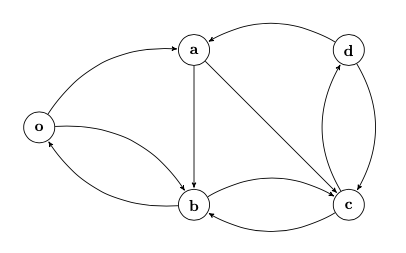
\includegraphics[width=0.5\columnwidth]{P1GivenGraph.png} % Example image
	\caption{Closed network in which particles move according to the transition rate matrix (\ref{eq:P1TransitioMatrix})}
	\label{fig:P1GivenGraph}
\end{figure}

\subsection*{Problem 3}
\begin{equation}
    \Lambda_{open} =\begin{pNiceMatrix}[first-row,last-col]
                    o & a & b & c & d\cr
                    0 & 2/3 & 1/3 & 0 & 0 & o \cr
                    0 & 0 & 1/4 & 1/4 & 2/4 & a \cr
                    0 & 0 & 0 & 1 & 0 & b \cr
                    0 & 0 & 0 & 0 & 1 & c \cr
                    0 & 0 &  0 & 0 & 0 & d 
                \end{pNiceMatrix}
    \label{eq:P3TransitioMatrix}
\end{equation}
\begin{figure}[H]
    \centering
	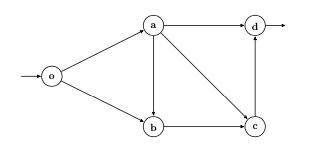
\includegraphics[width=0.5\columnwidth]{P3GivenGraph.png} % Example image
	\caption{Open network according to the transition matrix in (\ref{eq:P3TransitioMatrix})}
	\label{fig:P3GivenGraph}
\end{figure}




\section*{Problem 1 - Answer}
In the first part of this problem we are focusing on random walk of a particle in a weighted graph based on the transition probability $\Lambda$, basically we are talking about Markov chain in continuous time.
\begin{definition}[Random walk]
A random walk on a graph is a process that begins at some node, and at each time step moves to another node.
\end{definition}
\begin{definition}[Markov chain]
A stochastic process X(t) is said to be a \textbf{Markov chain} if satisfies the \textbf{Markov property}: the dependence of the future state on the history is limited to the present state.
\end{definition}
\begin{definition}[Continuous-time Markov Chain] \hspace{50pt}
\begin{itemize}
    \item[-] Given the Poisson process 
    \begin{equation}
        N_t := \sup{\left\{k \geq 0 : T_k \leq t\right\}}, \hspace{10pt} t \geq 0;
    \end{equation}
    \item[-] Given a finite state space $\mathcal{X}$ and a square nonnegative matrix $ \Lambda = (\Lambda_{ij})_{i,j \in \mathcal{X}} \neq 0$ with entries indexed by elements of $\mathcal{X}$ and diagonal entries $\Lambda_{ii} = 0$
    \item[-] Let:
    \begin{equation}
         w_i = \sum_{j\neq i}{\Lambda_{ij}}, \hspace{10pt} i \in \mathcal{X}, \hspace{10pt} w_{*} = \max_{i \in \mathcal{X}}{w_i} 
    \end{equation}
    
    \item[-] Consider a rate-$w_{*}$ Poisson clock $T0 \geq T1 \geq ...$ , the associated Poisson process $N_t$, and an independent discrete-time Markov chain $U(k), for k = 0, 1, ...$, with transition probabilities
    \begin{equation}
        \overline{P}_{ij} = \frac{\Lambda_{ij}}{w_{*}}, \hspace{10pt} i \in \mathcal{X}, \hspace{10pt}  \overline{P}_{ii} = \sum_{j\neq i}{\overline{P}_{ij}}
    \end{equation}
    The \textbf{discrete time Markov chain} is 
    \begin{equation}
        X(t) = U(N_t), \hspace{20pt} t\geq 0
    \end{equation} 
    where $N_t$ is called the jump chain associated to the continuous-time Markov chain $X(t)$.
\end{itemize}
\end{definition}
To accomplish the required task the \mintinline{python}{SimulateParticle} function has been built. That function will be used to produce simulations for both \emph{return time} and \emph{hitting times} estimation. 
\begin{enumerate}[(a\normalfont)]
    \item The average time obtained varies depending on the number of simulations computed, and it tends to the theoretical value computed at the point \emph{b)} as the number of simulations tends to infinite. 
    Some results obtained are in Table (\ref{tab:P1ReturnTimes}).
    
    \begin{table}[H]
      \begin{center}
        \begin{tabular}{r|c} 
          \textbf{\# of simulations} & \textbf{Avg return time}\\
          \hline
          1000 & 6.6865 \\
          10000 & 6.7037 \\
          100000 & 6.7362 \\
        \end{tabular}
      \end{center}
      \caption{Average return time on different number of simulations}
      \label{tab:P1ReturnTimes}
    \end{table}
    \item At this point we need to remark that the given grpah is \textbf{strongly connected}, and also we need to enunciate the following theorem
    \begin{theorem}\label{theo:P1ExpectedReturnTheo}
        Let $X(t)$ be a continuous-time Markov chain with finite state space $\mathcal{X}$ and transition rates $\Lambda_{ij} for i \neq j \in \mathcal{X}$. Let $\Lambda$ be the nonnegative square matrix with out-diagonal entries equal to the transition rates and diagonal entries $\Lambda_{ii} = 0$. 
        Let $\mathcal{G}_{\Lambda} = (\mathcal{X}; \mathcal{E}; \Lambda)$ be the graph with node set $\mathcal{X}$, and weight matrix $\Lambda$, and let $w = \Lambda \mathds{1}$, $P = diag(w)^1\Lambda$ be its degree vector and normalized weight matrix, respectively. 
        If $\mathcal{G}_{\Lambda}$ is strongly connected, then
        \begin{itemize}
            \item[...]
            \item[(iv)] the expected return times satisfies
            \begin{equation}\label{eq:ExpectedReturnTimesTheo}
                \mathds{E}_i[\overline{T}_{i}^{+}] = \frac{1}{w_i \overline{\pi}_i}
            \end{equation}
        \end{itemize}
        On the other hand, if $\mathcal{S} \in \mathcal{X}$ is a subset of states that is globally reachable in $\mathcal{G}_{\Lambda}$, then
        \begin{itemize}
            \item[(v)] the expected hitting times $\mathds{E}_i[T_\mathcal{S}]$ are the unique solution of
            \begin{equation}\label{eq:ExpectedHittingTimesTheo}
                \mathds{E}_{\mathcal{S}}[T_\mathcal{S}] = 0, \hspace{20pt} \mathds{E}_i[T_\mathcal{S}] = \frac{1}{w_i} + \sum_{j \in \mathcal{X}}{\overline{P}_{ij} \mathds{E}_{j}[T_\mathcal{S}]}, \hspace{20pt} i \in \mathcal{X}/\mathcal{S}
            \end{equation}
            \item[...]
        \end{itemize}
    \end{theorem}
    Calculating the expected return time on node \emph{a} as state in Theorem (\ref{theo:P1ExpectedReturnTheo}) Equation (\ref{eq:ExpectedReturnTimesTheo}) gives as result $\mathbf{\mathds{E}_i[\overline{T}_{i}^{+}] = 6.7500}$.
    
    As already said, if the number of simulations in point \emph{a)} tends to infinite their result will be closer to $\mathds{E}_i[\overline{T}_{i}^{+}]$.
    \item Again, the average hitting time obtained varies depending on the number of simulations computed, and it tends to the theoretical value explained at the point \emph{d)} as the number of simulations tends to infinite. 
    Some results obtained are in Table (\ref{tab:P1HittingTimes}).
    
    \begin{table}[H]
      \begin{center}
        \label{tab:table1}
        \begin{tabular}{r|c} 
          \textbf{\# of simulations} & \textbf{Avg hitting time}\\
          \hline
          1000 & 9.0984 \\
          10000 & 8.8634 \\
          100000 & 8.7432 \\
        \end{tabular}
      \end{center}
      \caption{Average hitting time of a particle that moves from node o to node d on different number of simulations}
      \label{tab:P1HittingTimes}
    \end{table}
    
    \item Hitting times can be computed as stated in Theorem (\ref{theo:P1ExpectedReturnTheo}) Equation (\ref{eq:ExpectedHittingTimesTheo}). The result obtained with the given graph and transition matrix, for a random walk from node $o$ to node $d$ is $\mathds{E}_{o}[T_d] =\mathbf{8.7857}$.
    
    \item Simulating the system as required we can see that the dynamics converge to a consensus. To explain that, we need some definitions. 
    \begin{definition}[French - De Groot opinion dynamics].\newline
        Consider a network described as a graph $\mathcal{G} = (\mathcal{V}, \mathcal{E}, W)$, where the node set $\mathcal{V}$ represents a population of agents, the link set $\mathcal{E}$ represents interactions among agents, and the entries $W_{ij}$ of the weight matrix quantify the strength of the influence that agent $j$ has on agent $i$. Let $P$ be the normalized weight matrix of $\mathcal{G}$. Assume that every agent $i$ has a state $x_i(t) \in \mathds{R}$ that is updated at discrete time steps $t = 0,1,...$ in response to the current states of her/his out-neighbors in $\mathcal{G}$ according to the following linear averaging rule
        \begin{equation}\label{eq:generalLinearAvgRule}
            x(t + 1) = Px(t), \hspace{20pt} t = 0,1,...
        \end{equation}
        where $x(t) = (x_i(t))_{i \in \mathcal{V}}$ is the vector of all agents' opinions. Equation (\ref{eq:generalLinearAvgRule}) is the \textbf{linear averaging dynamics on} $\mathbf{\mathcal{G}}$.
        In social science Equation (\ref{eq:generalLinearAvgRule}) is known as the \textbf{French-DeGroot opinion dynamics model}.
    \end{definition}
    \begin{proposition}
    Given a graph $\mathcal{G} = (\mathcal{V}; \mathcal{E};W)$ and $P = D^{-1}W$, consider the linear averaging dynamics (\ref{eq:generalLinearAvgRule}). The following facts hold true:
    \begin{itemize}
        \item[...]
        \item[(ii)] For every initial condition $x_0$, the evolution $x(t)$ satisfies
        \begin{equation}\label{eq:generalEvolutionWithPi}
            \pi^{'}x(t) = \pi^{'}x_0
        \end{equation}
        for every $\pi$ invariant distribution of $P$.
    \end{itemize}
    Suppose now that for an initial condition $x_0 \in \mathcal{R}^{\mathcal{V}}$ the evolution $x(t)$ determined by (\ref{eq:generalLinearAvgRule}) converges to some $\overline{x} \in \Omega$. Then, the following facts hold true:
    \begin{itemize}
        \item[(iii)] 
        \begin{equation}
            P\overline{x} = \overline{x}; \hspace{20pt} \pi^{'}x_0 = \pi^{'}\overline{x}
        \end{equation}
        for every $\pi$ invariant distribution of $P$.
        \item[(iv)] If, in addition, $s_\mathcal{G} = 1$,
        \begin{equation}\label{eq:xBarEqPiPrimeXZero}
            \overline{x} = \mathds{1}\pi^{'}x_0
        \end{equation}
        where $\pi$ is the unique invariant distribution of $P$
    \end{itemize}
    \end{proposition}
    \begin{proposition}\label{prop:propAlpha}
    Let $\mathcal{G}$ be a graph such that $s_{\mathcal{G}} = 1$ and the connected component of $\mathcal{G}$ corresponding to the unique sink of its condensation graph is aperiodic. Let $P$ be the normalized weight matrix of $\mathcal{G}$ and let $\pi = P^{'}\pi$ be its unique invariant probability. Then, the discrete-time averaging dynamics (\ref{eq:generalLinearAvgRule}) satisfies
    \begin{equation}\label{eq:consensusAlpha}
        \lim_{t \to +\infty}x(t) = \alpha\mathds{1}, \hspace{20pt} \alpha = \pi^{'}x(0)
    \end{equation}
    \end{proposition}
    
    In the given graph there are all conditions for which, through Proposition (\ref{prop:propAlpha}), we can affirm that for sure the \textbf{dynamics will converge to a consensus}, which value can be found with Equation (\ref{eq:consensusAlpha}). 
    
    In the practice in the script the initial state of each node is randomly determined using the function \mintinline{python}{numpy.random.rand}, then it is possible to compute the evolution of the French - De Groot dynamics and compare it with the theoretical value, obtaining the same result. 
    In Figure (\ref{fig:P1f}) we can see how the evolution of the simulated dynamics converge to the theoretical value of the consensus. 
    \begin{figure}[H]
        \centering
    	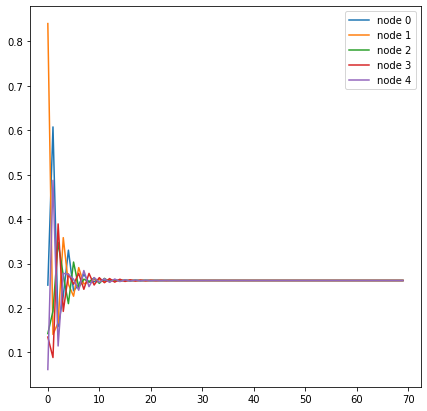
\includegraphics[width=0.5\columnwidth]{P1f.png} 
    	\caption{Convergence of the French - De Groot dyanmics }
    	\label{fig:P1f}
    \end{figure}
    
    \item We can assume that a community of agents is represented by the given graph $\mathcal{G} = (\mathcal{V}, \mathcal{E}, W)$ that is strongly connected and aperiodic and there is an underlying state of the world represented by a scalar parameter $\theta$, and every agent $i \in \mathcal{V}$ observes a noisy version of it, that corresponds with its initial opinion $x_i(0) = \xi_i$.
    
    $\{\xi_i \}_{i \in \mathcal{V}}$ are $i.i.d$ random variables, created in the practice with the function\newline \mintinline{python}{numpy.random.rand} that return values uniformly distributed between $0$ and $1$, with $\mathds{E}[\xi] = 0.5$ and $\sigma^2 = 1/12$. 
    We can consider now the initial states as 
    $$ x_i(0) = \xi_i = \theta + \psi_i $$
    where $\psi_i$ is the noise described above. 
    From the general theory we know that 
    $$ \overline{x} = \sum_{k \in \mathcal{G}}\pi_kx_k(0) = \theta + \sum_{k \in \mathcal{G}}\pi_k\psi_k $$
    where $\pi$ is the invariant distribution centrality of $\mathcal{G}$. $\overline{x}$ is thus a random variable whose expectation coincide with $\theta$, while its variance is 
    \begin{equation}\label{eq:xBarVar}
        \sigma^{2}_{\overline{x}} = \sigma^2 \sum_{k \in \mathcal{G}}\pi_k^2
    \end{equation}
    
    The theoretical value of the variance obtained with Equation (\ref{eq:xBarVar}) is $\sigma^{2}_{\overline{x}} = 0.0178$
    
    Simulating the French - De Groot dynamics on the given system we obtain a variance $\sigma^{2}_{\overline{x},sim} = 0.0171$ that is similar to the theoretical value $\sigma^{2}_{\overline{x}}$.
    
    Here it is also important to notice that the variance of the consensus is less than the variance of the initial opinion, meaning that the crowd is wiser than any single individual. This says that, as long as the graph describing the influence among individuals is connected and the individuals have all the same measurement capabilities (e.g. same error variance), the linear averaging dynamics always leads to an estimation of the true state $\theta$ that is strictly better than their original estimation.
    
    This case is known as \textbf{the wisdom of crowd}.
    
    \item Removing edges $(d,a)$ and $(d,c)$ the node $d$ become a sink node as in Figure (\ref{fig:P1Ga}), to simulate the French - De Groot dynamics we need to add a self-loop to the node $d$, as in Figure (\ref{fig:P1Gb}). Doing so, the node $d$ will not be influenced by other agents in the network, but will act as a \emph{stubborn} node. 
    In fact computing the invariant distribution $\pi$ we obtain as expected $\pi = [0, 0, 0, 0, 1]$, that indicate that the consensus value computed as in Equation (\ref{eq:consensusAlpha}) will depend only from the initial opinion of the node $d$. 
    Simulations computed sustain the previous assumption, as reported in Table (\ref{tab:P1ConsensusG}).
    
    \begin{table}[H]
      \begin{center}
        \begin{tabular}{c|c|c} 
          \textbf{Initial opinions} & \textbf{Empirical consensus} & \textbf{Theoretical consensus}\\
          \hline
          $ [10, 0, 0, 0, 1] $ & 1.0000 & 1\\
          $ [94, 43, 32, 1, 0] $ & 0.0000 & 0 \\
          $ [0.3703 0.5832 0.6985 0.2499 0.4909] $ & 0.4909 & 0.4909 
        \end{tabular}
      \end{center}
      \caption{Simulations with different initial states for the node $d$, initial opinions refers to nodes $[o, a, b, c, d]$}
      \label{tab:P1ConsensusG}
    \end{table}
    
    
    While, considering the initial opinions as random variables and computing the variance on the consensus value with $1000$ simulations we obtain $\sigma^2_{\overline{x}} = 0.0825$, much more closer to the variance of the of the initial opinion vector. 
    In fact at each simulation the the consensus will be the value of initial state of node $d$ and that value is chosen among a uniform distribution $\mathcal{U}(0,1)$ that has variance $\sigma^2 = 1/12$.
    
    \begin{figure}[H]
    \centering
        \begin{subfigure}{.5\textwidth}
            \centering
            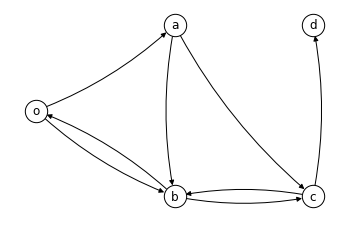
\includegraphics[width=1\linewidth]{P1Ga.png}
            \caption{Graph $\mathcal{G}$ with removed edges $(d,a)$ and $(d,c)$}
            \label{fig:P1Ga}
        \end{subfigure}%
        \begin{subfigure}{.5\textwidth}
            \centering
            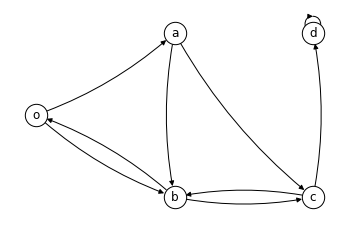
\includegraphics[width=1\linewidth]{P1Gb.png}
            \caption{Graph $\mathcal{G}$ with self-loop added on node $d$}
            \label{fig:P1Gb}
        \end{subfigure}
        \caption{}
        \label{fig:P1G}
    \end{figure}
    
    \item Again we start considering the graph in Figure (\ref{fig:P1GivenGraph}) and remove edges $(c,b)$ and $(d,a)$, and we obtain the graph in Figure (\ref{fig:P1H})
    
    \begin{figure}[H]
        \centering
    	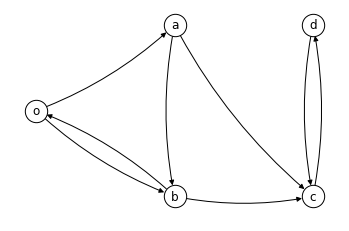
\includegraphics[width=0.3\columnwidth]{P1H.png} 
    	\caption{Graph obtained removing edges $(c,b)$ and $(d,a)$}
    	\label{fig:P1H}
    \end{figure}
    
    Randomly choosing the initial opinions, the French - De Groot dynamics \textbf{do not converge}. With a better look at the graph we can see that removing edges the graph is not connected anymore, in fact from the node $d$ we can only reach node $c$ and vice-versa. 
    Now the graph does not satisfy the requirements to calculate the consensus value with Equation (\ref{eq:consensusAlpha}), but the corresponding condensation graph has still only 1 sink. In this situation the only way to make the system reach a consensus, is to \textbf{give to all the node in the sink component the same initial opinion}, in this way the sink component nodes will act together as a sink node ad the French - De Groot dynamic will converge to their initial opinion. 
    Some simulations are reported in the Table (\ref{tab:P1ConsensusH}) and Figure (\ref{fig:P1Hconverge})
    
    \begin{table}[H]
      \begin{center}
        \begin{tabular}{c|c} 
          \textbf{Initial opinions} & \textbf{Empirical consensus} \\
          \hline
          $[0.4679, 0.3616, 0.2771, 1, 1]$ & 1\\
          $[0.8525, 0.4262, 0.6882, 7, 7]$ & 7\\
          $[0.1445, 0.7719, 0.3533, 4, 4]$ & 4\\
          $[0.2118, 0.3410, 0.5384, 2, 2]$ & 2
        \end{tabular}
      \end{center}
      \caption{Simulations with different initial states for the node $d$ and $c$, initial opinions refers to nodes $[o, a, b, c, d]$}
      \label{tab:P1ConsensusH}
    \end{table}
    
    \begin{figure}[H]
        \centering
    	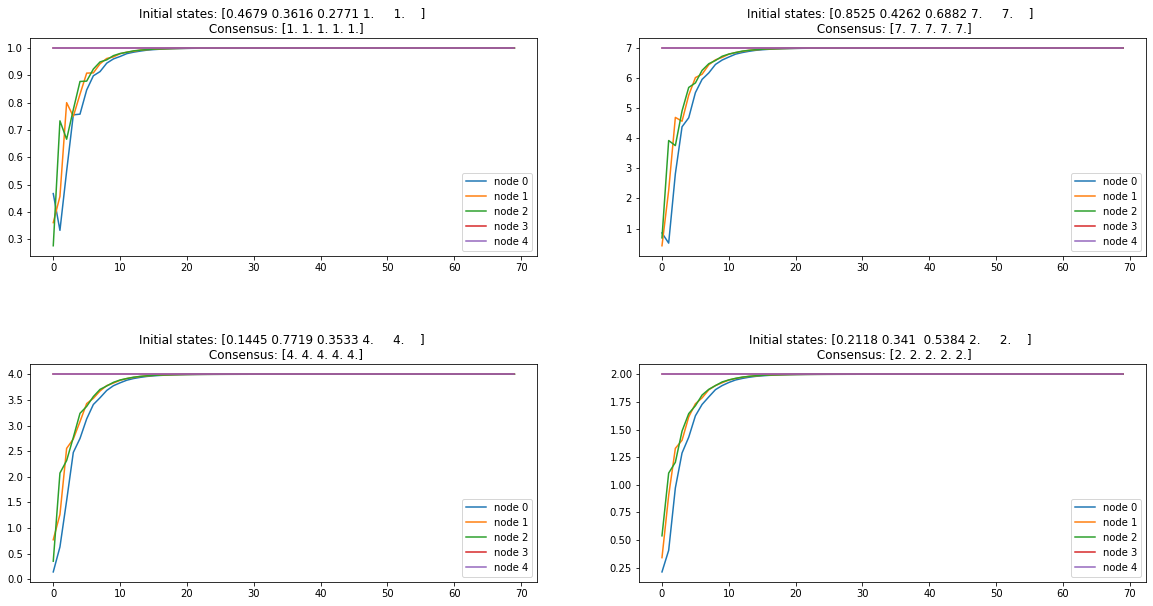
\includegraphics[width=0.8\columnwidth]{P1Hconverge.png} 
    	\caption{Convergence to a consensus when nodes $c$ and $d$ are at the same initial opinion}
    	\label{fig:P1Hconverge}
    \end{figure}
\end{enumerate}

\section*{Problem 2}
In this problem we are considering again the graph in figure (\ref{fig:P1GivenGraph}) with weights according to (\ref{eq:P1TransitioMatrix}).
\begin{enumerate}[(a\normalfont)]
    \item We want to observe the average return times of 100 particles starting from node $a$. To do so, the function \mintinline{python}{particlePerspectiveParticleClock} has been built. The average return time on the node $a$ over $100$ particles is 
    $$ \overline{T}_a^+ = 6.7890$$
    and we can see how close this value is to the theoretical return time found in \emph{Problem 1 Point b} ($\mathds{E}_i[\overline{T}_{i}^{+}] = 6.7500$).
    \item To answer the first question the function \mintinline{python}{NodePerspectiveGlobalClock} has been built, with this function we can simulate \mintinline{python}{nParticles} moving in the graph during \mintinline{python}{time} units of time for \mintinline{python}{nSimulations} simulations. 
    At the end we can compute the average of the number of particles in each node at the end, across all simulations. 
    In the Figure (\ref{fig:P2b}) we can see the evolution during the simulation time of the number of particles in each node. 
    \begin{figure}[H]
        \centering
    	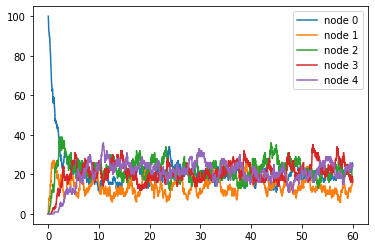
\includegraphics[width=0.8\columnwidth]{P2b.png} 
    	\caption{Number of particles in node during time of simulation}
    	\label{fig:P2b}
    \end{figure}
    
    The average number of particle in each node at the end of the simulations is
    $$
    \begin{bNiceMatrix}[first-row]
        o & a & b & c & d\cr
        18.74 & 14.92 & 22.50 & 22.30 & 21.54
    \end{bNiceMatrix}
    $$
    
    If we divide the obtained average by the number of particles put in the graph we obtain 
    $$
    \begin{bNiceMatrix}[first-row]
        o & a & b & c & d\cr
        0.1874 & 0.1492 & 0.2250 & 0.2230 & 0.2154
    \end{bNiceMatrix}
    $$
    that is pretty similar to the stationary distribution of the continuous-time random walk followed by the single particles computed in Problem 1.
    $$
    \begin{bNiceMatrix}
    0.1851 & 0.1481 & 0.2222 & 0.2222 & 0.2222
    \end{bNiceMatrix}
    $$
\end{enumerate}

\section*{Problem 3}
We consider now the open network in Figure (\ref{fig:P3GivenGraph}) with transition rate matrix $\Lambda_{open}$ in (\ref{eq:P3TransitioMatrix}).
Particles will enter the system at node $o$ according to a Poisson process with rate $\lambda = 1$ and each node will then pass along a particle according to a specific rate.

\begin{enumerate}[a)\normalfont]
    \item \textbf{Proportional rate:}\newline
    In this first part the rate of the Poisson clock of each node is equal to the number of particles in it.
    The system has been simulated for 60 time units giving as result the evolution in Figure (\ref{fig:P3a1}), then the input rate $\lambda$ has been increased at $10$, $100$ and $500$ obtaining the evolution in Figures (\ref{fig:P3a2}) (\ref{fig:P3a3}) (\ref{fig:P3a4}). 
    The system does not blow up, in fact we can see how particles  keep distributing across all nodes even when the input rate $\lambda$ increases. 
    
    \begin{figure}
    \centering
        \begin{subfigure}{0.7\textwidth}
            \centering
            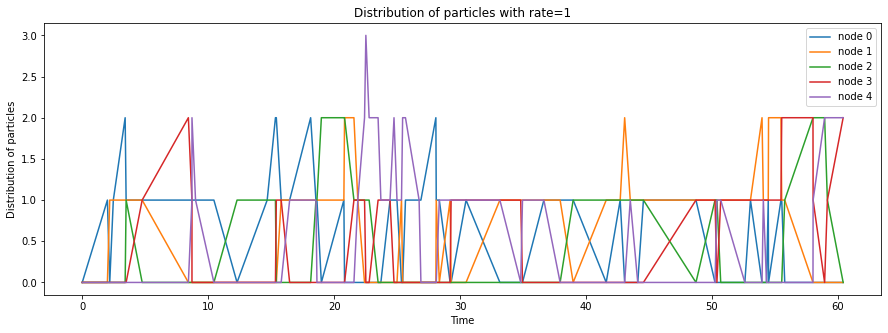
\includegraphics[width=1\linewidth]{P3a1.png}
            \caption{(Particle perspective) Distribution of particles across node during simulation time, input rate = $1$}
            \label{fig:P3a1}
        \end{subfigure}
        \begin{subfigure}{0.7\textwidth}
            \centering
            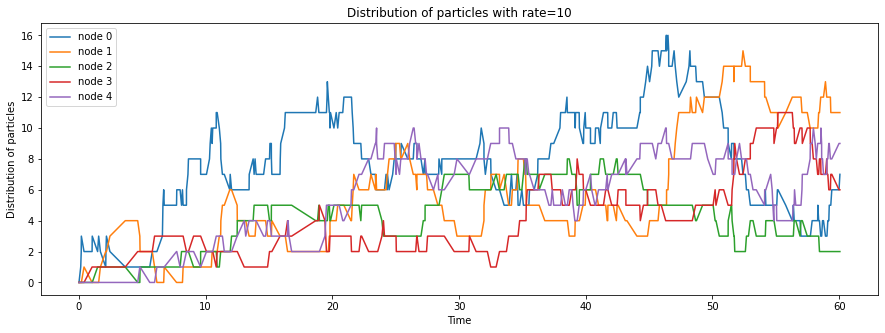
\includegraphics[width=1\linewidth]{P3a2.png}
            \caption{(Particle perspective) Distribution of particles across node during simulation time, input rate = $10$}
            \label{fig:P3a2}
        \end{subfigure}
        \begin{subfigure}{0.7\textwidth}
            \centering
            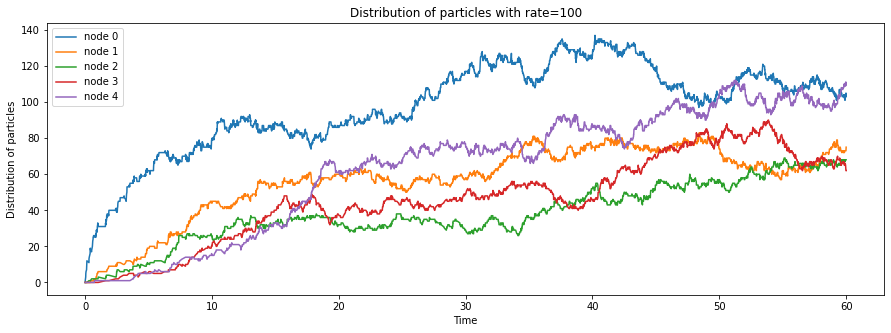
\includegraphics[width=1\linewidth]{P3a3.png}
            \caption{(Particle perspective) Distribution of particles across node during simulation time, input rate = $100$}
            \label{fig:P3a3}
        \end{subfigure}
        \begin{subfigure}{0.7\textwidth}
            \centering
            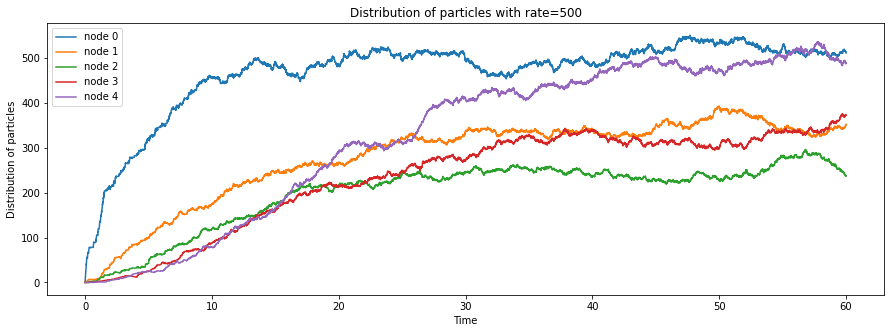
\includegraphics[width=1\linewidth]{P3a4.png}
            \caption{(Particle perspective) Distribution of particles across node during simulation time, input rate = $500$}
            \label{fig:P3a4}
        \end{subfigure}
        \caption{}
        \label{fig:P3a}
    \end{figure}
    
    \item \textbf{Proportional rate:}\newline
    In this part the rate of the Poisson clock of each node is fixed, and equal to one. Again we simulate it for 60 time units obtaining the distribution of particles in Figure (\ref{fig:P3b1}). The the input rate has been increased to $10$ and $100$ with result in Figures (\ref{fig:P3b2}) (\ref{fig:P3b3}). We can notice that with input rate $100$ the particles are all accumulated in the starting node $o$ and have difficulty to distribute across other nodes, in particular we have $0$ particles in node $d$. The system has blown up now. 
    
    After a further investigation we can find that this behavior of the system starts with an input rate $\lambda = 30$ when about the $80\%$ of particles in the system at the end of the simulation is still in the node $o$, as we can see in Figure (\ref{fig:P3blow}).
    
    \begin{figure}
    \centering
        \begin{subfigure}{0.9\textwidth}
            \centering
            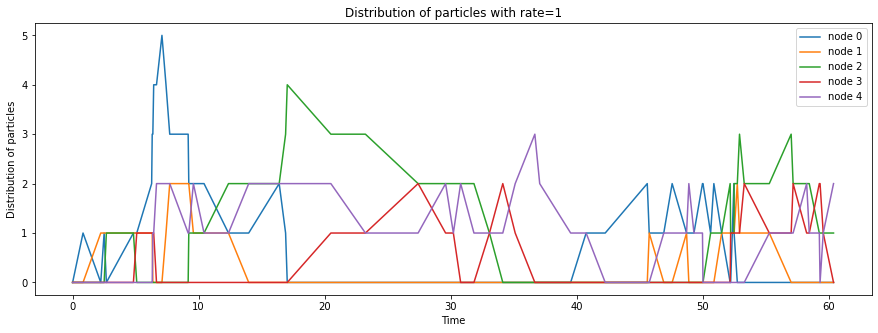
\includegraphics[width=1\linewidth]{P3b1.png}
            \caption{(Node perspective) Distribution of particles across node during simulation time, input rate = $1$}
            \label{fig:P3b1}
        \end{subfigure}
        \begin{subfigure}{0.9\textwidth}
            \centering
            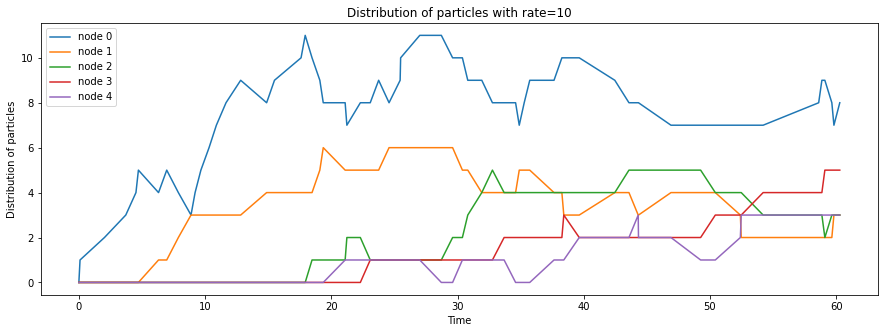
\includegraphics[width=1\linewidth]{P3b2.png}
            \caption{(Node perspective) Distribution of particles across node during simulation time, input rate = $10$}
            \label{fig:P3b2}
        \end{subfigure}
        \begin{subfigure}{0.9\textwidth}
            \centering
            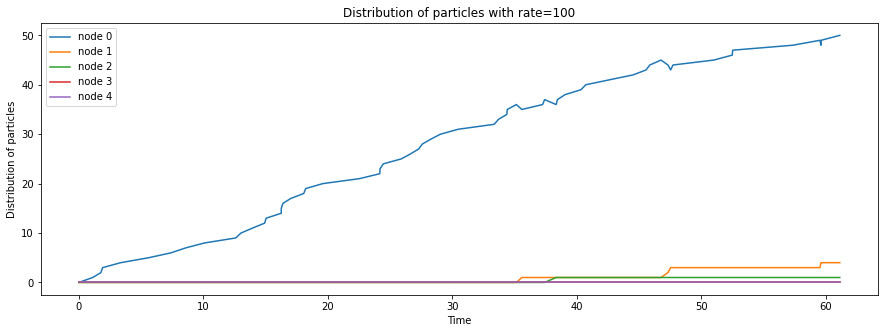
\includegraphics[width=1\linewidth]{P3b3.png}
            \caption{(Node perspective) Distribution of particles across node during simulation time, input rate = $100$}
            \label{fig:P3b3}
        \end{subfigure}
        \caption{}
        \label{fig:P3b}
    \end{figure}
    
    \begin{figure}[H]
        \centering
    	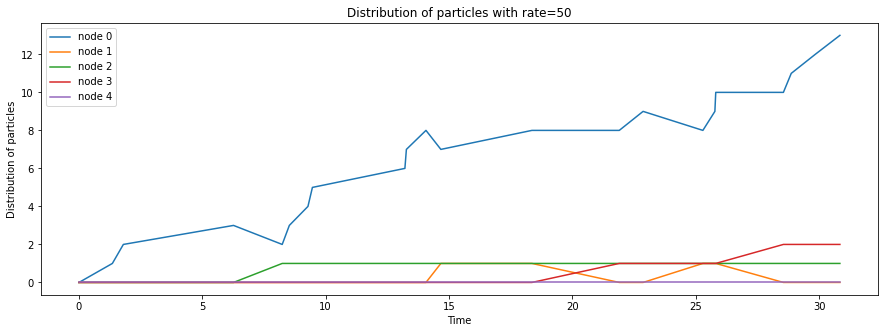
\includegraphics[width=0.8\columnwidth]{P3blow.png} 
    	\caption{(Node perspective) System starts blowing up with input rate $\lambda = 30$}
    	\label{fig:P3blow}
    \end{figure}
    
\end{enumerate}


%----------------------------------------------------------------------------------------

\end{document}
